\documentclass[a4paper,10pt]{report}

\usepackage{graphicx}
\usepackage{color}

\usepackage{caption}
\usepackage{subcaption}

\usepackage[portuguese]{babel}
\usepackage[utf8]{inputenc}
\usepackage[T1]{fontenc}

\usepackage{geometry}
\geometry{a4paper}
\usepackage[parfill]{parskip}

\usepackage{changepage}

\usepackage{amsmath}

\usepackage{fancyhdr}


\graphicspath{{./imagens/}}

\usepackage{url}
\usepackage{lastpage}
\usepackage{lscape}
\usepackage{verbatim}
\usepackage{fancyvrb}
\usepackage{listings}
\usepackage{float}

\usepackage[colorlinks=true,linkcolor=blue,citecolor=blue]{hyperref}

\lstset{
    extendedchars=\true,
    inputencoding=utf8
}

\renewcommand{\lstlistingname}{Código}
\usepackage{color}
\definecolor{grey}{rgb}{0.9,0.9,0.9}
\definecolor{greyD}{rgb}{0.5,0.5,0.5}

\lstnewenvironment{code}[1][]%
{
   \noindent
   \lstset{
  float=htpb,
  backgroundcolor=\color{grey},
  basicstyle=\scriptsize,
  numbers=left,
  numbersep=5pt,
  numberstyle=\tiny\color{greyD},
  breaklines=true,
  frame=single,
  #1}
}
{}

\begin{document}


\begin{titlepage}
\begin{center}

\begin{flushleft}

\includegraphics[height=3.00cm]{EENG.jpg}\\
\end{flushleft}

\vspace{1.5cm}

\Large{\textbf{LEI --- Licenciatura de Engenharia Informática}}\\
\vspace{1cm}
\Large{\textbf{Processamento de Linguagens}}\\

\vspace{1cm}

\Huge{\textbf{Compilador de uma LPIS}} \\

\vspace{2cm}

\Large{\textbf{Orlando Costa -  a67705, Paulo Araujo - a58925, Rui Oliveira - a67661}}\\
\begin{figure}[h]
\centering
\begin{subfigure}{.3\textwidth}
  \centering
  
\includegraphics[width=\textwidth]{Orlando.jpg}
\end{subfigure}
\begin{subfigure}{.3\textwidth}
  \centering
  
\includegraphics[width=\textwidth]{Paulo.jpg}
\end{subfigure}
\begin{subfigure}{.3\textwidth}
  \centering
  
\includegraphics[width=\textwidth]{Oliveira.jpg}
\end{subfigure}
\end{figure}

\vspace{1.5cm}
Braga, 7 de Junho de 2015

\end{center}

\end{titlepage}


\begin{abstract}
Este relatório descreve o desenvolvimento de um compilador para uma linguagem de programação imperativa simples (LPIS). 

A linguagem desenvolvida foi baseada na linguagem de programação C, e suporta:
\begin{itemize}
  \item Variáveis globais
  \item Ciclos: for, while, do while
  \item Estruturas de Condição: If .. Else
  \item Expressões Aritméticas e lógicas
  \item Funções com argumentos
  \item Declaração de variáveis locais dentro das funções
\end{itemize}
O compilador foi desenvolvido com recurso ao analisador léxico Flex e ao analisador sintático Yacc.

\end{abstract}
%----------------------------------------------------------------------
%\newpage
%\phantom{placeholder} % doesn't appear on page
%\thispagestyle{empty} % if want no header/footer
%----------------------------------------------------------------------
\tableofcontents
\pagenumbering{arabic}

%\phantom{placeholder} % doesn't appear on page
%----------------------------------------------------------------------
%\newpage
%\phantom{placeholder} % doesn't appear on page
%\thispagestyle{empty} % if want no header/footer
%----------------------------------------------------------------------
%\pagestyle{fancy}
%\setlength{\headheight}{15.2pt}
%\fancyhf{} % apagar as configurações actuais
%\fancyfoot[LE,RO]{\thepage}
%\fancyhead[LE,RO]{PL - Trabalho Pratico 1 --- Araujo P., Belo O., Oliveira R.}
%\page{setcounter}{0}
%----------------------------------------------------------------------

\chapter{Introdução}
\label{cap:intro}
O presente trabalho enquadra-se na unidade curricular de Processamento de Linguangens da Licenciatura em Engenharia Informática da Universidade do Minho. O trabalho pretende aumentar a experiência em engenharia de linguagens, e motivar a utilização de ferramentas de compilação de compiladores e análise léxica.

Para isso era pretendido criar uma linguagem de programação imperativa simples, que será descrita à frente.
O compilador desta linguagem foi desenvolvido desde a analise léxica até à geração de código. O Código gerado foi assembly para a maquina virtual fornecida por o docente.


\section{Linguagem de programação imperativa simples}
    Previamente ao desenvolvimento do compilador existe a necessidade de definir uma linguagem sobre a qual este atua, com base numa qualquer linguagem imperativa. Neste sentido e por simplicidade e familiaridade, a linguagem de programação C é a selecionada. Esta linguagem foi simplificada por forma a adaptar-se aos requisitos propostos, sofrendo as seguinte modificações na sua estrutura:
\begin{itemize}

    \item Apenas permite manusear variáveis do tipo inteiro (escalar ou array).
    \item Suporta apenas as instruções vulgares de controlo de fluxo de execução (condicional e cíclica), tais como if-else, for, while e do-while.
    \item As instruções que controlam inserção e output de valores (tipicamente printf e scanf) estão adaptadas para suportar apenas inteiros, e então estão renomeadas (printi e scani).
    \item As expressões lógicas devem estar rodeadas por parentises para facilitar a sua distinção e ordem quando em conjunto com expressões aritméticas. 
\end{itemize}


\section{Arquitetura}
    O sistema desenvolvido é principalmente constituído por 2 modelos: parser.l e compiler.y, que são respetivamente o analisador léxico e analisador sintático. 

    Na Figura \ref{fig:dependencias}, é possível observar as dependências entre os diversos ficheiros.

    O analisador sintático utiliza o ficheiro vmCompiler.h, sendo que este modulo responsável pelo tratamento das variáveis e funções existentes (adicionar/consultar variáveis).

    O sistema utiliza também duas estruturas de dados: uma HashMap e uma Stack. A hashmap é utilizada para guardar as variáveis e as funções, enquanto que a stack permite o controlo das labels dos ciclos durante a compilação.

    Na figura \ref{fig:struct} é possível observar as estruturas utilizadas em vmCompiler:
    \begin{itemize}
      \item Scope - possui uma map com a informação das variáveis, onde a chave é nome da variável e o valor é um EntryVar;
      \item EntryFun - guarda a informação sobre o tipo de uma função (argumentos de entrada e tipo de retorno);
      \item EntryVar - guarda o tipo, nome o endereço relativo de uma dada variável.
    \end{itemize}

    Analisadas as estruturas referidas, de notar as variáveis criadas em vmCompiler, representadas na figura \ref{fig:objs}, onde é possível observar duas variáveis do tipo Scope, uma para o contexto global e outra para o contexto interior a uma função.

    Finalmente, existe um map de EntryFun (mFuncMap) onde a chave é o nome da função, e a variável DecFunAux consiste num apontador temporário para uma função declarada.

\begin{figure}
\centering
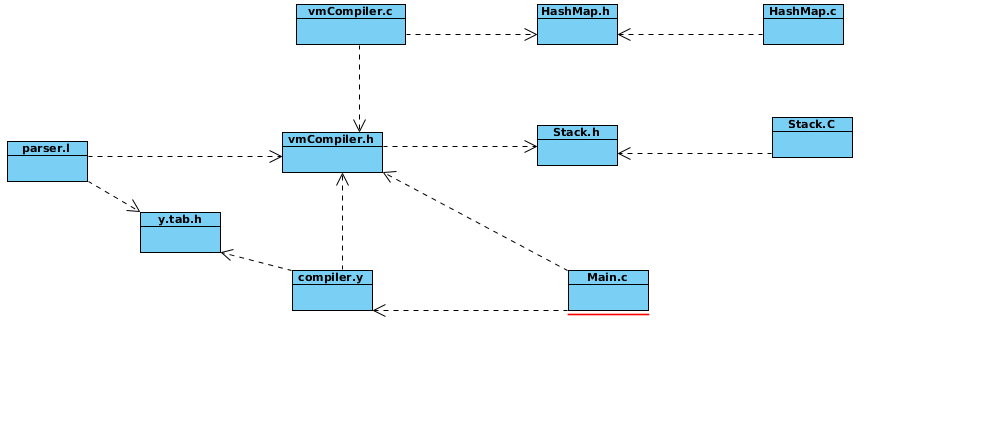
\includegraphics[width=15cm]{imagens/dependecias.png}
\caption{Diagrama das pedendencias dos ficheiros}
\label{fig:dependencias}
\end{figure}

\begin{figure}
\centering
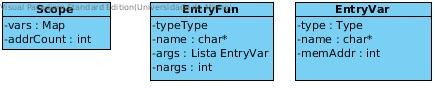
\includegraphics[width=10cm]{imagens/estruturas.jpg}
\caption{Diagrama das estruturas usadas em vmCompiler}
\label{fig:struct}
\end{figure}

\begin{figure}
\centering
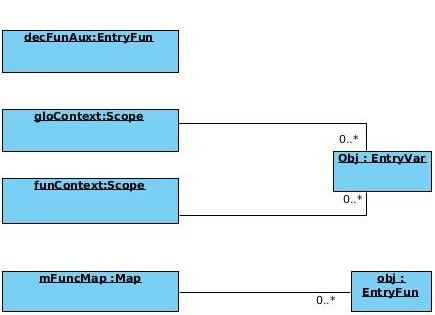
\includegraphics[width=10cm]{imagens/objetos.jpg}
\caption{Diagrama dos objetos existente em vmCompiler}
\label{fig:objs}
\end{figure}



\section{Estruturas de dados}

\subsection{Stack}
      De forma a evitar confusão na atribuição de \emph{labels} relativas a \emph{ifs} e \emph{loops} é utilizado um contador de condições. À medida que é encontrada uma instrução que implique o uso de uma condição, este contador é incrementado e o seu valor é colocado numa stack. Deste modo, o valor que se encontra no topo da stack é relativo ao último \emph{ciclo/if} encontrado. Sempre que é encontrado o final de uma condição, o valor no topo da stack é removido. Através do uso de um contador e de uma stack, é muito mais simples gerir as \emph{labels} e as operações de controlo, como \emph{JUMPs} e \emph{JZs}.
      A stack utilizada implementa apenas as funções necessárias para a sua inicialização, inserção, remoção e consulta. Com as operações de push/pop são inseridos/removidos valores no topo da stack, e com a operação de get apenas é consultado o valor no topo da stack, sem que este seja removido. Esta última operação é útil para a geração de instruções 'JZ' na geração de código VM.

\subsection{HashMap}
	Como foi referido anteriormente, é utilizada uma \emph{hashmap} com o objetivo de guardar as variáveis e as funções. Quanto às variáveis, é necessário guardar e aceder a informação como o seu endereço e tipo. Sendo assim, foi criada uma estrutura de dados auxiliar para armazenar essa informação. O nome da variável é utilizado como chave e, a partir dela, conseguimos aceder à sua informação correspondente na hashmap. 
	Relativamente às funções, é necessário guardar e aceder a informação como o seu nome, informação relativa aos seus argumentos de entrada e o tipo de dados de saída. Para esse feito, também foram necessárias estruturas de dados auxiliares como uma lista ligada capaz de armazenar informação relativa aos argumentos de entrada e uma outra que contem a informação relativa ao tipo de dados de saída, dados de entrada e nome da função. Neste caso, o nome da função funciona como chave na \emph{hashmap} e o seu valor é a estrutura que contem a informação mais geral sobre a função.
	A \emph{hashmap} utilizada implementa funções necessárias para a sua inicialização, inserção, remoção e consulta, sendo que também contém outras funções que não foram utilizadas no desenvolvimento deste projeto.


\chapter{Compilador}


\section{Analisador léxico}
  O analisador léxico encontra-se desenvolvido com o suporte da ferramenta 'ylex' e deteta todos os símbolos terminais da linguagem (palavras reservadas, sinais e variáveis). Este analisador efetua também a deteção de comentários (linhas precedidas pelos símbolos '//'), ignorando o texto neles contidos. De forma a facilitar a deteção os erros de sintaxe, o parser conta as linhas que já interpretou. Este funcionalidade permite ao analisador sintático informar a linha onde ocorrer a anomalia em caso de erro de processamento. A passagem de valores é efetuada através do yylval.  

\section{Analisador sintático/semântico}

O analisador sintático/semântico é o responsável por processar os tokens obtidos através do analisador léxico, 
utilizando as produções definidas para calcular a instrução a escrever no ficheiro de output final. O ficheiro onde se encontram todas as 
produções denomina-se compiler.y, 

\begin{description}

\item[Definição dos tokens] \hfill \\

Previamente à definição das produções, estão definidos os diversos tokens assim como o tipo das diferentes variáveis presentes nas produções. Encontram-se também definidas as precedências correspondentes às operações aritméticas, assim como a produção inicial (Prog).  

\item[Produções iniciais] \hfill \\

O processamento é iniciado na produção Prog, correspondente ao começo do programa. São realizadas as inserções iniciais no ficheiro de output, e as produções a serem efetuadas podem consistir numa lista de declarações, numa lista de funções, ou numa lista de instruções. Caso se encontre uma lista de declarações, é realizado o controlo de saltos de instruções, através da inserção da instrução "JUMP init" no ficheiro de output. Isto possibilita a declaração de variáveis antes da declaração das funções, de forma a que as funções possuam acesso às variáveis globais declaradas.  

\item[Produções de Funções] \hfill \\

A declaração de funções é precedida pelo símbolo terminal '\#', de forma a facilitar a sua leitura e distinção com outras instruções. O armazenamento das funções declaradas é realizado através da utilização de uma hashmap, e permite guardar o contexto de estas, ou seja, as declarações efetuadas dentro da função são tidas como variáveis locais, e apenas acessíveis dentro da função. No final da declaração da função, o contexto é encerrado. Por simplicidade, não é possível utilizar chamadas a funções como argumento de outra função.

\item[Produções de declarações] \hfill \\

As declarações de variáveis podem ocorrer dentro do contexto de uma função (i.e. variáveis locais) ou fora de qualquer contexto (i.e. variáveis globais). Desta forma, ao declarar uma variável, é efetuada o teste que verifica se está está declarada ou não dentro de uma função. Além disso, não é permitido re-declarar variáveis locais com o mesmo nome que variáveis globais já existentes, sendo apresentado um erro quando isso ocorre.

\item[Produções de instruções e atribuições] \hfill \\

São suportadas diversas instruções, no entanto vale a pena mencionar a instrução "return". Esta instrução calcula o endereço a retornar a partir do número de argumentos de entrada da função na qual se insere e do frame pointer salvaguardado. As atribuições permitem efetuar o incremento/decremento de variáveis através da sintaxe var++/var--, assim como atribuir o valor de expressões a variáveis escalares ou vetoriais. 
\item[Produções de input/output] \hfill \\

As produções referentes à leitura e escrita no stdin. A produção de escrita suporta a impressão de expressões, sendo que a produção de leitura armazena as variáveis atribuídas conforme o contexto definido. 

\item[Produções de controlo de fluxo de execução condicional] \hfill \\

A instrução de controlo de fluxo de execução condicional está definida como if...else, suportando um conjunto de instruções no seu contexto.

\item[Produções de controlo de fluxo de execução cíclico] \hfill \\

As produções correspondentes ao controlo de fluxo de execução cíclico suportam ciclos 'while', 'do while' e 'for'. Estas produções são suportadas por uma estrutura de dados (stack), sendo graças a esta que é possível calcular o saltos a efetuar.

\item[Produções de cálculo de expressões] \hfill \\

O compilador possui a capacidade de processar expressões aritméticas e lógicas, tanto em forma de declaração como em forma de cálculo do índice de um array. Estas expressões possibilitam também a utilização de parêntesis aninhados.

\end{description}

Nota: Na compilação do código referente ao programa yacc, é apresentado um erro de compilação do tipo shift-reduce. No entanto, este erro não provoca qualquer comportamento indesejado no programa dado que por defeito, quando em dúvida, o yacc efetua um shift ao invés de um reduce, sendo este o comportamento pretendido para este caso.


\section{Geração de código máquina}
A cada regra da gramática, são associadas ações a serem executadas à medida que estas são reconhecidas. Assim sendo, é realizada uma tradução da linguagem desenvolvida para a linguagem \emph{assembly} da VM, à medida que cada instrução ou expressão é identificada. A maioria destas ações implica uma instrução de escrita no ficheiro de output. Todas estas acções que implicam escrita no ficheiro são triviais, existindo apenas algumas exceções como o caso do ciclo 'for'.
No ciclo 'for', é necessária a utilização de instruções 'JUMP', de forma a ser possível seguir o seu fluxo de execução normal. Após a identificação e execução das ações associadas à expressão lógica presente no ciclo 'for', é gerado o salto condicional respetivo, assim como um salto para as instruções associadas ao corpo do ciclo. Além disso, é gerada uma \emph{label} que irá corresponder ao incremento do ciclo que irá ser identificado de seguida. Identificado o final do corpo do ciclo, é efetuado um salto para a \emph{label} correspondente ao incremento do ciclo, que para além das respetivas instruções, conterá outro 'JUMP' para o teste da expressão lógica.

\subsection{Funções}

De forma a implementar adequadamente o processamento de funções, é necessário resolver certas implicações, sendo que esta funcionalidade obriga a tratar de diversos contextos dentro do programa (global e local).

As declarações das funções são efetuadas após as declarações das variáveis globais para que dentro das funções seja possível aceder às variáveis globais.

As declarações de variáveis são feitas no inicio da função, e no hash table das variáveis é guardado não apenas o endereço mas também o contexto (local ou global). Desta forma, no acesso às variáveis, utiliza-se 'PUSHG' ou 'PUSHL' seja respetivamente variável global ou local.

A passagem de argumentos para a função é tratada como uma declaração especial na qual o endereço é negativo. Já o retorno da função é colocado também num endereço negativo que foi previamente alocado na chamada da função.

Em forma de exemplo, assumindo a chamada de uma função com 2 argumentos. Como é possível observar na figura \ref{fig:functionStack}, os endereços são negativos ao fp, e o endereço onde a função colocará o retorno é $fp - 3$.
Após a execução da função é feito o 'pop' dos argumentos e assim o valor de retorno da função está no topo da stack. 

\begin{figure}
\centering
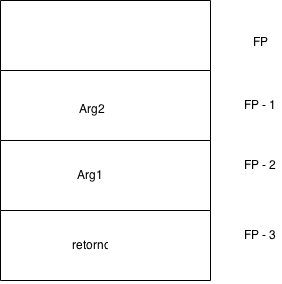
\includegraphics[width=5cm]{functionStack.png}
\caption{Chamada de uma função}
\label{fig:functionStack}
\end{figure}

\chapter{Testes}
\subsection{Teste 1}
\subsubsection{Input}
\lstinputlisting[language=c]{anexos/t1.in}
\subsubsection{Output}
\lstinputlisting[language=c]{anexos/t1.out}


\subsection{Teste 2}
\subsubsection{Input}
\lstinputlisting[language=c]{anexos/t2.in}
\subsubsection{Output}
\lstinputlisting[language=c]{anexos/t2.out}



\subsection{Teste 3}
\subsubsection{Input}
\lstinputlisting[language=c]{anexos/t3.in}
\subsubsection{Output}
\lstinputlisting[language=c]{anexos/t3.out}


\subsection{Teste 4}
\subsubsection{Input}
\lstinputlisting[language=c]{anexos/t4.in}
\subsubsection{Output}
\lstinputlisting[language=c]{anexos/t4.out}

\subsection{Teste 5}
\subsubsection{Input}
\lstinputlisting[language=c]{anexos/t5.in}
\subsubsection{Output}
\lstinputlisting[language=c]{anexos/t5.out}


\chapter{Conclusão}
\label{cap:intro}

Finalizado o desenvolvimento do trabalho, é possível analisar o resultado final e o impacto que as diversas decisões tiveram sobre este. Um dos principais pontos positivos consiste na implementação do processamento e compilação de funções, sendo esta a funcionalidade mais trabalhosa e sobre a qual recaiu maior parte do tempo despendido. Relativamente a estas, de notar uma mudança na forma como estas foram implementadas. Anteriormente, a estrutura relativa ao armazenamento de dados de uma função possuía a capacidade de dar acesso às variáveis declaradas dentro do seu contexto, no entanto decidiu-se que esta funcionalidade era desnecessária para o funcionamento do compilador, sendo esta informação descartada. A implementação das expressões de controlo de execução possuíram também uma dificuldade acrescida, obrigando à utilização de estruturas de dados mais complexas, tais como hashmaps e stacks. Creemos ter alcançado os objetivos definidos aquando da proposta do trabalho, tendo desenvolvido um compilador capaz de processar uma LPIS, com a possibilidade de dar feedback sobre o código de input definido e criar o ficheiro com instruções em Assembly correspondentes.


\chapter{Anexos}
\section{parser.l}
\lstinputlisting[language=c]{anexos/parser.l}
\section{compiler.y}
\lstinputlisting[language=c]{anexos/compiler.y}
\section{vmCompiler.c}
\lstinputlisting[language=c]{anexos/vmCompiler.c}


\end{document}




% respectivo enunciado, da descricao do problema, das decisoes que lideraram o desenho da solucao e sua implementacao (incluir a especificacao Flex , deverao conter exemplos de utilizacao (textos fontes diversos e respectivo resultado produzido)